\Chapter{Resultaten\label{hfdst-resultaten}}

In dit hoofdstuk zullen verscheidene ASIC implementaties van de schakeling, die in \refhfdst{hfdst-implementatie} beschreven werd, van naderbij bestudeerd worden. Daarbij zal gelet worden op de oppervlakte en het vermogenverbruik van het resultaat. Er zal onderzocht worden wat het effect van de verschillende voorgestelde optimalisaties is op deze parameters. Ten slotte zal het ontwerp vergeleken worden met reeds bestaande implementaties.

\section{Gebruikte software}

Het ontwerp werd geprogrammeerd in GEZEL \cite{gezel}. Simulaties en compilatie naar VHDL werden uitgevoerd met GEZEL 2.0. De optimalisaties werden manueel uitgevoerd in de VHDL code, aangezien dit in GEZEL niet mogelijk was.

Alle ontwerpen werden gesynthetiseerd met behulp van Synopsys Design Vision (versie Y-2006.06). De gebruikte bibliotheek was de \emph{$0.13 \mu m$ low leakage} bibliotheek van Faraday Technology \cite{cell-databook}. De maximale oppervlakte werd ingesteld op nul, wat als netto effect een resultaat met minimum oppervlakte gaf. Verder werd voor het kloksignaal, indien niet anders vermeld, een frequentie van 10 kHz gebruikt.

\section{Gerapporteerd vermogen}

Voor de resultaten in verband met vermogenverbruik worden steeds twee waarden gegeven. De eerste waarde, dynamisch vermogen, geeft weer hoeveel vermogen verbruikt wordt door veranderende CMOS in- en uitgangen. De tweede waarde, lekvermogen, is vermogenverbruik dat voorkomt zelfs indien er geen signalen van waarde veranderen. De impact hiervan hangt onder meer af van de gebruikte bibliotheek. Het is voor het syntheseprogramma zeer moeilijk een nauwkeurige schatting voor het vermogenverbruik te geven, dus de gegeven waarden moeten niet als exact worden beschouwd.

Indien gewenst kan het vermogenverbruik voor hogere kloksnelheiden geschat worden. Gegeven de standaard frequentie $f = 10$ kHz, de formule voor het dynamisch vermogen van een CMOS schakeling:
\[P_d = V^2 \cdot C \cdot f\]
en het lekvermogen $P_l$, kan men het totale vermogen omrekenen naar dat van een willekeurige kloksnelheid via
\[P' = \frac{P_d \cdot f'}{10 \cdot 10^3} + P_l.\]
Het verkregen resultaat zal niet volledig kloppen, maar komt zeer dicht in de buurt van het door Design Vision geschatte verbruik.

\section{Benodigde rekentijd}

Alvorens de syntheseresultaten te presenteren, wordt even uitgewijd over het noodzakelijk aantal klokcycli $c$ om \'e\'en pairing te berekenen. Merk op dat de formules die volgen enkel kloppen voor willekeurige $m$ indien $\textsf{Hamm}(l) = 3$, wat het geval is voor de gekozen parameters (zie \refsect{sectie-implementatie-parameters}).

Het totaal aantal cycli voor een schakeling met veldgrootte $m$ en aantal MALU's $d$ wordt gegeven door:
\[c = 21681 + 4322 + 2998 \cdot \left\lceil \frac{m}{d} \right\rceil.\]
Daarbij staat het eerste getal voor het aantal klokcycli waarin gegevens van plaats verschoven worden in het intern geheugen. Het tweede getal is het aantal optellingen dat uitgevoerd dient te worden en de co\"efficient voor de vermenigvuldiging is het aantal vermenigvuldigingen. Het aantal klokcycli $c$ kan verder opgesplitst worden in het aantal cycli $c_f$ voor de for-lus en $c_m$ voor de finale machtsverheffing. In dat geval zijn de formules:
\[\begin{gathered}
c_f = 18731 + 3937 + 2463 \cdot \left\lceil \frac{m}{d} \right\rceil\\
c_m = 2950 + 385 + 535 \cdot \left\lceil \frac{m}{d} \right\rceil,
\end{gathered}\]
waarbij de co\"efficienten opnieuw voor respectievelijk geheugenverschuivingen, optellingen en vermenigvuldigingen staan.

In \reftbl{tabel-resultaten-multi-cycles} wordt voor enkele waarden getoond hoeveel klokcycli nodig zijn om een berekening te voltooien in het geval $m = 163$. In \reffig{figuur-resultaten-multi-cycles} wordt hetzelfde weergegeven, maar dan voor elke $d$ van 1 t.e.m.\ 163. Het is duidelijk dat de tijdsbesparing dankzij extra MALU's vrij snel teniet wordt gedaan door het aantal cycli dat niet door $d$ be\"invloed wordt.

\begin{table}[h]
	\caption{Aantal klokcycli $c$ nodig voor \'e\'en pairing i.f.v.\ het aantal MALU's $d$ voor veldgrootte $m = 163$}
	\label{tabel-resultaten-multi-cycles}

	\begin{narrow}{-1cm}{-1cm}
		\centering
		\begin{tabular}{lllllllll}
			\toprule
			$d$	& 1	& 2	& 3	& 4	& 6	& 8	& 16	& 32\\
			$c$	& $514\,677$	& $271\,839$	& $190\,893$	& $148\,921$	& $109\,947$	& $88\,961$	& $58\,981$	& $43\,991$\\
			\bottomrule	
		\end{tabular}
	\end{narrow}
\end{table}

\begin{figure}[h]
	\centering
		\fbox{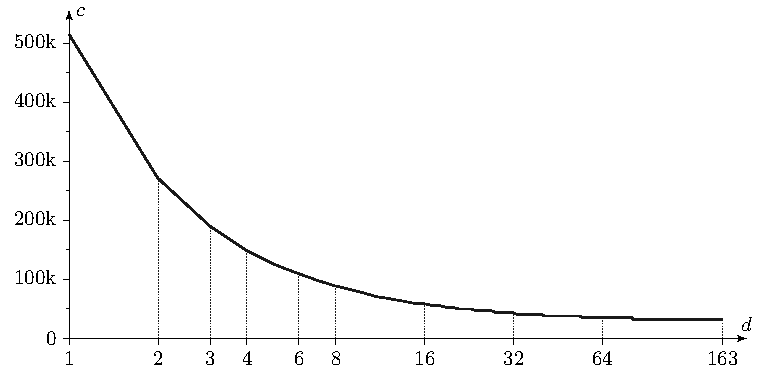
\includegraphics[width=11.9cm]{results-multi-cycles}}
		\caption{Aantal klokcycli $c$ nodig voor \'e\'en pairing i.f.v.\ het aantal MALU's $d$ voor veldgrootte $m = 163$\label{figuur-resultaten-multi-cycles}}
\end{figure}

\section{Basisimplementatie \& optimalisaties\label{section-resultaten-basisimplementatie}}

Logischerwijs wordt eerst gekeken naar de syntheseresultaten voor een implementatie met \'e\'en MALU. Verder zal in deze paragraaf ook onderzocht worden wat de effecten zijn van de optimalisaties voorgesteld in \refsect{sectie-implementatie-optimalisaties}. Bij de implementaties met clock gating werden steeds ook de resetingangen van zoveel mogelijk registers verwijderd. Ten slotte zal onderzocht worden hoeveel oppervlakte de individuele onderdelen van het ontwerp innemen.

De syntheseresultaten voor de vijf verschillende implementaties worden gegeven in \reftbl{tabel-resultaten-optimalisaties}. De versies met clock gating (CG~$n$) implementeren de schakelingen in de volgorde waarin ze voorkomen in \refsect{subsectie-implementatie-optimalisatie-clock-gating}. Ter verduidelijking zijn deze resultaten ook nog eens uitgezet in \reffig{figuur-resultaten-m1}.

%De synthese software gebruikt in de basis implementatie en die zonder resetingangen flip flops met een enable ingang. Zo'n flip flops kosten achtentwintig gates, waarbij de resetingang door twee van die gates gevormd wordt. Intern zijn deze flip flops equivalent aan een flip flop zonder enable ingang die naar zichzelf is terug gekoppeld via een multiplexer. Het enable signaal vervult in dit geval de functie van selectie signaal die anders voor de multiplexer nodig zou zijn. De synthese software zal zelf de sturing van de enable signalen bepalen in dit gevallen. Het is om deze reden dat het toepassen van clock gating in dit geval geen oppervlakte winst oplevert tegenover.

\begin{table}[h]
	\caption[Syntheseresultaten voor implementaties met \'e\'en MALU]{Syntheseresultaten voor implementaties met \'e\'en MALU. CG staat voor clock gating, de nummering komt overeen met de volgorde van de clock gating schakelingen in \refsect{subsectie-implementatie-optimalisatie-clock-gating}.}
	\label{tabel-resultaten-optimalisaties}

	\centering
	\begin{tabular}{llrlrlr}
		\toprule
		\multirow{2}{*}{Ontwerp}	& \multicolumn{2}{l}{\multirow{2}{*}{Opp. [gates]}}	& \multicolumn{4}{c}{Vermogen @ 10 kHz [$nW$]}\\
		\cmidrule{4-7}
		&	& & \multicolumn{2}{c}{Dynamisch}	& \multicolumn{2}{c}{Lek}\\
		\midrule
		Basis			& $28\,876$	& 			& 512	&	 		& 117 & \\
		Geen Reset	& $27\,596$	& 96\%	& 395	& 77\%	& 107 & 92\%\\
		CG 1			& $27\,751$	& 96\%	& 94	& 18\%	& 109	& 94\%\\
		CG 2			& $27\,713$	& 96\%	& 59	& 12\%	& 102	& 88\%\\
		CG 3			& $27\,734$	& 96\%	& 96	& 19\%	& 110	& 94\%\\
		\bottomrule		
	\end{tabular}
\end{table}

\begin{figure}[h]
	\centering
		\fbox{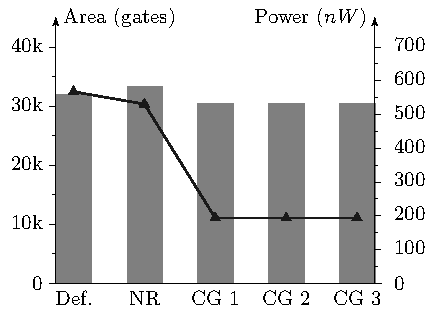
\includegraphics[scale=1]{results-m1}}
		\caption[Syntheseresultaten voor implementaties met \'e\'en MALU en $f = 10$ kHz]{Syntheseresultaten voor implementaties met \'e\'en MALU en $f = 10$ kHz. GR staat voor geen reset, CG staat voor clock gating, de nummering komt overeen met de volgorde van de clock gating schakelingen in \refsect{subsectie-implementatie-optimalisatie-clock-gating}.\label{figuur-resultaten-m1}}
\end{figure}

Zoals verwacht resulteert het toepassen van clock gating in een zeer grote besparing op het vermogen. Het is zelfs zo dat na toepassing van clock gating het dynamisch vermogen lager is dan het lekvermogen. Daarbij dient opgemerkt te worden dat het dynamisch vermogen zal stijgen bij een hogere kloksnelheid terwijl het lekvermogen constant zal blijven.

Het is opmerkelijk dat het dynamisch vermogen van CG~2 zo veel lager wordt gerapporteerd dan dat van de andere twee CG implementaties. Hoe dit komt, is moeilijk  te zeggen. In werkelijkheid zal implementatie CG~3 het minste verbruiken. 

Verder valt het ook op dat de implementaties met clock gating niet kleiner zijn dan die zonder. Normaal gezien zou de toepassing van deze schakeling per register \'e\'en multiplexeringang moeten elimineren. Waarom de synthesesoftware dit niet doet, is onduidelijk. Er werd getracht de synthesesoftware zelf clock gating te laten implementeren, maar de resulterende implementatie was noch kleiner, noch minder verbruikend dan het niet-geoptimaliseerde ontwerp.

%clock gating methode drie bespaart enkel energie tegenover de andere methodes indien de ingang van een register wijzigt wanneer dat register geen nieuwe waarde moet opslaan. De enige ingang die echter vaak wijzigt is die van het register verbonden met de uitgang van de $\mathbb{F}_{2^m}$ kern tijdens een vermenigvuldiging. Zolang een vermenigvuldiging aan de gang is, moet ditzelfde register echter telkens zijn eigen waarde verschoven met \'e\'en positie naar links opslaan. Met andere woorden: op het moment dat de clock gating schakeling zijn besparende werk zou kunnen verrichten, wordt het register sowieso elke klokslag beschreven met een nieuwe waarde. Het effect is dus dat in dit geval de schakeling effectief geen of amper vermogensbesparing teweeg brengt tegenover de andere clock gating schakelingen. Verder is het ook goed mogelijk dat de synthese software bij het berekenen van het verbruik niet nauwkeurig genoeg tewerk gaat om het effect van de schakeling op de interne gates van de flip flop in rekening te kunnen brengen.

Ten slotte wordt nog ontleed hoeveel oppervlakte de individuele onderdelen van de schakeling innemen. \reftbl{tabel-resultaten-onderdelen} geeft een overzicht van de grootte van de verschillende delen van implementatie CG~3. Het valt op dat de zestien registers en de FSM, die bestaat uit 553 toestanden, samen goed zijn voor 95,5\% van de oppervlakte. Het effect daarvan zal duidelijk worden in de volgende paragraaf, wanneer meerdere MALU's ge\"implementeerd worden.

\begin{table}[h]
	\caption{Oppervlakte van de individuele onderdelen in de implementatie met \'e\'en MALU}
	\label{tabel-resultaten-onderdelen}

	\centering
	\begin{tabular}{llr}
		\toprule
		Onderdeel					& \multicolumn{2}{c}{Opp. [gates]}\\
		\midrule
		MALU				 			& 458			& 1,7\%\\
		$\mathbb{F}_{2^m}$ kern	&				& \\
		$\quad$ Logica				& 783			& 2,8\%\\
		$\quad$ Registers			& 962			& 3,5\%\\
		Controller					&				& \\
		$\quad$ Logica				& $13\,044$	& 47\%\\
		$\quad$ Registers			& $12\,487$	& 45\%\\
		\midrule
		Totaal						& $27\,734$	& 100\%\\
		\bottomrule		
	\end{tabular}
\end{table}


\section{Meerdere MALU's\label{sectie-resulaten-MALU's}}

Mits de toevoeging van extra MALU's is het, zoals aangetoond, mogelijk de totale rekeningtijd drastisch te verlagen. Hoewel het gebruik van meerdere MALU's de uiteindelijke schakeling vergroot en dat dus enigszins in gaat tegen de originele doelstelling, wordt hier toch onderzocht in welke mate de interessante parameters hierdoor juist worden be\"invloed.

Op de implementaties met meerdere MALU's werd steeds de derde clock gating techniek (en het verwijderen van resetingangen) toegepast, aangezien dit in werkelijkheid de grootste energiebesparing teweeg zou moeten brengen. Implementaties met een aantal MALU's gaande van twee t.e.m.\ twee\"endertig werden gesynthetiseerd. Een nog hoger aantal MALU's zou immers compleet ingaan tegen de originele doelstelling.

De resultaten van de synthese zijn te zien in \reftbl{tabel-resultaten-md} en \reffig{figuur-resultaten-md}. Zoals in de vorige paragraaf gezien, neemt een MALU zeer weinig oppervlakte in in de implementatie. Het toevoegen van een klein aantal extra MALU's brengt dus weinig extra oppervlakte en vermogenverbruik met zich mee. Het is dus een aangeraden manier om de snelheid van de schakeling op te drijven. Dit wordt nog verder onderzocht in de volgende paragraaf. Het gerapporteerde dynamisch verbruik van de implementatie met twee MALU's is lager dan dat van de implementatie met \'e\'en MALU, dit is opnieuw een fout van de software.

\begin{table}[h]
	\caption{Syntheseresultaten voor implementaties met $d$ MALU's}
	\label{tabel-resultaten-md}

	\centering
	\begin{tabular}{llrlrlrl}
		\toprule
		\multirow{2}{*}{$d$} & \multicolumn{2}{l}{\multirow{2}{*}{Opp. [gates]}}	& \multicolumn{4}{c}{Vermogen @ 10 kHz [$nW$]}	& \multirow{2}{*}{$\begin{array}{@{}c@{}}\text{Tijds-}\\\text{winst}\end{array}$}\\
		\cmidrule{4-7}
		&	& & \multicolumn{2}{c}{Dynamisch}	& \multicolumn{2}{c}{Lek}	&\\
		\midrule
		1			& $27\,734$	& 			& 96	& 			& 110	& 			& \\
		2			& $28\,423$	& 102\%	& 90	& 94\%	& 113	& 103\%	& 47,2\%\\
		3			& $29\,071$	& 105\%	& 103	& 107\%	& 118	& 107\%	& 62,9\%\\
		4			& $30\,278$	& 109\%	& 108	& 113\%	& 122	& 111\%	& 71,1\%\\
		6			& $30\,956$	& 112\%	& 112	& 117\%	& 127	& 115\%	& 78,6\%\\
		8			& $32\,782$	& 118\%	& 122	& 127\%	& 136	& 124\%	& 82,7\%\\
		16			& $37\,798$	& 136\%	& 162	& 169\%	& 163	& 148\%	& 88,5\%\\
		32			& $47\,833$	& 172\%	& 212	& 221\%	& 213	& 194\%	& 91,5\%\\
		\hline		
	\end{tabular}
\end{table}

\begin{figure}[h]
	\centering
		\fbox{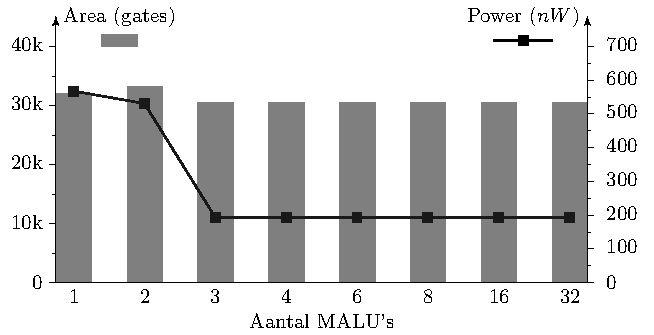
\includegraphics[scale=1]{results-md}}
		\caption{Syntheseresultaten voor implementaties met meerdere MALU's en $f = 10$ kHz\label{figuur-resultaten-md}}
\end{figure}

\section{Hogere kloksnelheid vs.\ meerdere MALU's}

Aan een kloksnelheid $f = 10$ kHz doet een schakeling met \'e\'en MALU er 51.5 seconden over om \'e\'en pairing te berekenen. Dit zal  in de meeste gevallen onaanvaardbaar zijn. Daarom wordt hier onderzocht wat de effecten op de schakeling zijn indien de kloksnelheid wordt opgedreven en er eventueel meerdere MALU's gebruikt worden. Ter illustratie zal voor een implementatie met meerdere MALU's die met twee nader onderzocht worden. Opnieuw wordt in beide gevallen clock gating schakeling drie gebruikt en worden zoveel mogelijk resetingangen verwijderd.

Stel een maximale rekentijd $t_{\text{max}} \approx 50$ $ms$. Voor een implementatie met \'e\'en MALU moet de klokfrequentie $f_1$ dan 1030 maal verhoogd worden. Wanneer men de schakeling met twee MALU's even snel wenst te maken als die met \'e\'en dan dient de kloksnelheid $f_2$ van die eerste vermenigvuldigd te worden met $\Delta f = 1 - 0,472$. De kloksnelheden van de respectievelijke schakelingen zijn dan:
\[\begin{aligned}
f_1	&\approx 10,3\text{ MHz}\\
f_2	&\approx 5,44\text{ MHz}.
\end{aligned}\]

Ter vergelijking worden de resulterende parameters van beide implementaties gegeven in \reftbl{tabel-resultaten-m1-vs-m2}. Beiden werden gehersynthetiseerd met aangepaste parameters voor de klok. Dat de schakeling met \'e\'en MALU in dit geval kleiner is dan in het geval $f = 10$ kHz, is te wijten aan enige willekeurigheid in de algoritmes van de synthesesoftware.

Hoewel de implementatie met twee MALU's 3\% groter is dan die met \'e\'en, verbruikt ze slechts half zoveel vermogen. Het lijkt dus vanzelfsprekend om steeds voor een implementatie met meerdere MALU's te kiezen indien de snelheid moet opgedreven worden. Hoeveel MALU's ideaal zijn, zal afhankelijk zijn van de toepassing.

\begin{table}[h]
	\caption{Vergelijking van syntheseresultaten voor twee verschillende implementaties met dezelfde uitvoeringstijd voor \'e\'en pairing}
	\label{tabel-resultaten-m1-vs-m2}

	\centering
	\begin{tabular}{lll@{$\;\;$}l}
		\toprule
		& 1 MALU	& \multicolumn{2}{l}{2 MALU's}\\
		\midrule
		$f$ [MHz]					& 10,3						& 5,44						& 53\% \\ 
		Opp. [gates]				& $27\,430$					& $28\,155$					& 103\% \\
		Vermogen [$\mu W$]		& 								& 								& \\
		$\quad$ Dynamisch			& 98,2						& 48,5						& 49\% \\
		$\quad$ Lek					& $107 \cdot 10^{-3}$	& $111 \cdot 10^{-3}$	& 104\% \\
		\bottomrule	
	\end{tabular}
\end{table}

\section{Vergelijking met bestaande implementaties}

Gezien de vrij recente ontdekking van pairings is het beschikbare aantal implementaties voor ASIC's ook vrij beperkt. Er werden slechts drie papers in de literatuur gevonden waarin het voorgestelde ontwerp naar een ASIC gesynthetiseerd werd. Op andere implementaties werd reeds ingegaan in \refsect{inleiding-pairings}.

De drie ASIC ontwerpen worden voorgesteld in respectievelijk \cite{beuchat-asic}, \cite{kammler} en \cite{savas}. Zowel in \cite{beuchat-asic} als \cite{savas} wordt met het oog op het behalen van zo hoog mogelijke snelheden ontworpen. De implementatie uit \cite{kammler} bevat naast de schakeling voor pairings tevens een RISC processor. In \cite{savas} wordt de finale machtsverheffing niet uitgevoerd. \reftbl{tabel-resultaten-asic} geeft een vergelijkend overzicht van het ontwerp voorgesteld in deze thesis en de vermelde ontwerpen. Aangezien het ontwerp uit \cite{beuchat-asic} het enige is waarvan alle gegevens bekend zijn, zal in de tekst die volgt enkel met dat ontwerp vergeleken worden. 

\begin{table}[h]
	\caption{Vergelijking van de implementatie voorgesteld in deze thesis met ASIC implementaties uit de literatuur}
	\label{tabel-resultaten-asic}

	\begin{narrow}{-2cm}{-2cm}
		\centering
		\begin{tabular}{llllll}
			\toprule
			&	\multicolumn{2}{c}{Thesis (CG 3)\footnotemark[2]}	& \multirow{2}{*}{$\begin{array}{@{}c@{}}\text{Pairing-}\\\text{Lite \cite{beuchat-asic}}\end{array}$}	& \multicolumn{1}{c}{\multirow{2}{*}{$\begin{array}{@{}c@{}}\text{Kammler}\\\text{\emph{et al.} \cite{kammler}}\end{array}$}}	&  \multicolumn{1}{c}{\multirow{2}{*}{$\begin{array}{@{}c@{}}\text{K\"om\"urc\"u en}\\\text{Savas \cite{savas}}\end{array}$}}\\
			\cmidrule(r){2-3}
			& \multicolumn{1}{c}{1 MALU} & \multicolumn{1}{c}{2 MALUs} & & &\\
	 		\midrule
			Veld																				& $\mathbb{F}_{2^{163}}$	& $\mathbb{F}_{2^{163}}$	& $\mathbb{F}_{3^{97}}$	& $\mathbb{F}_{p}$ 256 bit	& $\mathbb{F}_{3^{97}}$ \\
%			Veiligheid [bit]																& 652								& 652								& 922							& ?								& 922\\
			Pairing																			& Tate							& Tate							& $\eta_T$					& Ate			 					& Tate\\
			Technologie																		& 0,13 $\mu m$					& 0,13 $\mu m$					& 0,18 $\mu m$				& 0,13 $\mu m$					& 0,25 $\mu m$\\
			Opp. [gates]																	& $27\,734$						& $28\,155$						& $193\,765$				& $97\,000$						& \emph{$10 mm^2$}\footnotemark[3]\\
			$f$ [MHz]																		& 0,01							& 5,44							& 200							& 338								& 78\\
			Rekentijd [$\mu s$]															& $51,5 \cdot 10^6$			& $50 \cdot 10^3$				& 46,7						& $15,8 \cdot 10^3$			& 250\footnotemark[4]\\
			Vermogen [$mW$]																& $206 \cdot 10^{-6}$		& $48,6 \cdot 10^{-3}$		& 672							& \emph{onbekend}				& \emph{onbekend}\\
%			Score $\left[ mJ \cdot \text{gates} \right]$\footnotemark[4]	& 284								& 382								& 162							& ?								& ?\\
%			Score $\left[ \frac{nW}{\text{MHz} \cdot \text{gate}} \right]$\footnotemark[4]	& 0.74	& 0.32							& 17.34						& ?								& ?\\
%			Score $\left[ \frac{\text{fJ}}{\text{gate}} \right]$\footnotemark[4]	& 0,74					& 0,32							& 17,34						& ?								& ?\\
			\bottomrule		
		\end{tabular}
	\end{narrow}
	
	\footnotesize \footnotemark[2] Implementatie zonder resets en met toepassing van clock gating schakeling drie.
	
	\footnotemark[3] De gegeven oppervlakte is die van de complete schakeling inclusief routing.
	
	\footnotemark[4] Exclusief de finale machtsverheffing.
	
%	\footnotemark[4] Des te lager de score, des te conservatiever springt de implementatie om met energie. De score wordt berekend als score $= \frac{\text{verbruik}}{\text{frequentie} \cdot \text{oppervlakte}}$. 
\end{table}

Alvorens te vergelijken moet er uiteraard wel op gewezen worden dat het ontwerp uit \cite{beuchat-asic} zoals reeds vermeld niet ontworpen is met compactheid of laag vermogenverbruik in gedachten. Het is dus zeker niet de bedoeling het ontwerp af te breken. 

De hier voorgestelde implementaties zijn niet alleen ongeveer een factor zeven kleiner dan degene voorgesteld in \cite{beuchat-asic}, hun vermogenverbruik is ongelofelijk veel lager. Het energieverbruik per bit veiligheid, ofwel de energie-effici\"entie, kan berekend worden als:
\[\text{EE} = \frac{\text{vermogen} \times \text{rekentijd}}{\text{veiligheid}}.\]
Opgegeven waarden voor veiligheid zijn zeer veranderlijk van paper tot paper. In dit geval zullen waarden gebruikt worden die door de auteurs van \cite{beuchat-asic} worden opgegeven in \cite{beuchat}. Daar wordt gesteld dat het ontwerp uit deze thesis een veiligheid heeft van 652 bit en dat van \cite{beuchat-asic} 922 bit.

De resultaten van de berekening zijn te zien in \reftbl{tabel-resultaten-energie}. Er dient op gewezen te worden dat in het ontwerp uit \cite{beuchat-asic} met de $\eta_T$ pairing gewerkt wordt, die ongeveer een factor twee sneller berekend kan worden. Het is duidelijk dat het ontwerp uit deze thesis het potentieel heeft veel effici\"enter te zijn. Het gebruik van meer MALU's doet de de effici\"entie duidelijk stijgen. Dit is te verklaren door het feit dat meer MALU's relatief gezien zeer weinig extra vermogen verbruiken, maar de rekentijd wel gevoelig verlagen. Indien een iets grotere oppervlakte dus geen bezwaar is, kan de effici\"entie van de schakeling nog flink verhoogd worden door meer MALU's toe te voegen. Tevens kan, indien een lange rekentijd geen punt is, tegelijkertijd de frequentie verlaagd worden, wat de effici\"entie nog meer ten goede zal komen. 

\begin{table}[h]
	\caption{Vergelijking van energie-effici\"entie van de implementatie voorgesteld in deze thesis met ASIC implementaties uit de literatuur}
	\label{tabel-resultaten-energie}

	\begin{narrow}{-2cm}{-2cm}
		\centering
		\begin{tabular}{llll}
			\toprule
			&	\multicolumn{2}{c}{Thesis (CG 3)\footnotemark[2]}	& \multirow{3}{*}{$\begin{array}{@{}c@{}}\text{Pairing-}\\\text{Lite \cite{beuchat-asic}}\end{array}$}\\
			\cmidrule(r){2-3}
			& \multicolumn{1}{c}{$\begin{array}{@{}c@{}}d = 1,\\f = 10\text{kHz}\end{array}$} & \multicolumn{1}{c}{$\begin{array}{@{}c@{}}d = 2,\\f = 5.44\text{MHz}\end{array}$} &\\
	 		\midrule
			Vermogen [$mW$]																& $206 \cdot 10^{-6}$		& $48,6 \cdot 10^{-3}$		& 672\\
			Rekentijd [$\mu s$]															& $51,5 \cdot 10^6$			& $50 \cdot 10^3$				& 46,7\\
			Veiligheid [bit]																& 652								& 652								& 922\\
			Effici\"entie $\left[ \frac{nJ}{\text{bit}}\right]$\footnotemark[3]	& 16,3					& 3,73							& 34,0\\
			\bottomrule		
		\end{tabular}
	\end{narrow}
		
	\footnotesize \footnotemark[2] Implementatie zonder resets en met toepassing van clock gating schakeling drie.
	
	\footnotemark[3] Des te lager, des te conservatiever springt de implementatie om met energie.
\end{table}

Het is duidelijk dat de ontwerpen voorgesteld in deze thesis met kop en schouders uitsteken boven andere gepubliceerde ontwerpen indien compactheid en laag vermogen- en/of energieverbruik prioriteit genieten.
